  % -*- coding: utf-8 -*-
% !TeX encoding = UTF-8
% !TeX root = ../report.tex


%%%%%%%%%%%%%%%%%%%%%%%%%%%%%%%%%%%%%%%%%%%%%%%%%%%%%%%%%%%
\chapter{Datamateriale \label{kapitel_metode_datamateriale}}
%%%%%%%%%%%%%%%%%%%%%%%%%%%%%%%%%%%%%%%%%%%%%%%%%%%%%%%%%%%

Lorem ipsum dolor sit amet, consectetur adipisicing elit, sed do eiusmod
tempor incididunt ut labore et dolore magna aliqua. Ut enim ad minim veniam,
quis nostrud exercitation ullamco laboris nisi ut aliquip ex ea commodo
consequat. Duis aute irure dolor in reprehenderit in voluptate velit esse
cillum dolore eu fugiat nulla pariatur. Excepteur sint occaecat cupidatat non
proident, sunt in culpa qui officia deserunt mollit anim id est laborum.

%%%%%%%%%%%%%%%%%%%%%%%%%%%%%%%%%%%%%%%%%%%%%%%%%%%%%%%%%%%
\section{DISCO}
%%%%%%%%%%%%%%%%%%%%%%%%%%%%%%%%%%%%%%%%%%%%%%%%%%%%%%%%%%%


Datamaterialet er registerdata fra Danmarks Statistik%
% %
% 		\footnote{ Danmarks Statistik politik om datafortrolighed forlanger at alle tabeller med celler med under 3 observationer sættes til 0 for at hindre identifikation af enkeltindivider. Det lever denne afhandling naturligvis op til.}%
% %
i perioden 1996-2009. Danmarks Statistik (DST) benytter sig af den internationale klassifieringsstand for erhverv, ISCO (\emph{the International Standard Classification of Occupations}), der er udviklet af International Labour Organisation. ISCO findes i en lettere modificeret dansk udgave ved navn DISCO. Dette er den helt centrale variabel i min afhandling, af åbenlyse grunde. Den indeholder meget detaljerede oplysinger om beskæftigelse, og vil blive gennemgået i det følgende. 

Derefter vil en række andre variable berøres kort. En bortfaldsanalyse er at finde i bilag XX \#todo, og har konklusionen, at der ikke er årsag til bekymrig blah blah  

Populationen består af de 5.860.440 personer, der var beskæftigede på det danske arbejdsmarked i mindst ét af årene i perioden 1996-2009, og som var mellem 16 og 69 år. I gennemsnit var 2.340.300 mennesker i denne alder beskæftiget om året på det danske arbejdsmarked. Perioden er behandlet som et tværsnit, hvor alle skift mellem jobs i de 14 år benyttes i en mobilitetsmatrice. 



Det er naturligvis ikke alle, der skifter jobs. I gennemsnit skifter 313.073 personer jobs om året, i perioden, svarende til 13 \%.  Ved at lægge alle jobskifte i perioden sammen, er antallet af observerede skift i perioden 4.383.028. 

Det er ikke alle, der er observeret flere gange, da eksempelvis en person, der er 3 år gammel i 1996, godt kan nå at få et job som 16-årig i 2008, og skifte til et nyt job i 2009, uden at være med nogle af de andre år. 



At det er netop disse 14 år, skyldes: 1) databrud og uregelmæssigheder mellem 1995 og 1996 i en række baggrundsvariable såsom timeløn og ledighed 2) DISCO-klassifikationssystemet har et væsentlig databrud i 2010, hvor DISCO-88-versionen opgraderes til DISCO-08 versionen. På det detaljeringsniveau af DISCO, jeg arbejder på, har det ikke været muligt at finde en tilfredsstillende sammenkobling mellem de to DISCO-versioner.

Perioden dækker heldigivs en nogenlunde stabil periode i dansk økonomi, der var præget af økonomisk fremgang, og denne afhandling kan derfor siges at beskrive det danske arbejdsmarked i en opgangsperiode (find tal på det her, økonomisk årbog, fx \#todo)

Der bruges alene data fra DISCO-koder, som har mere end xxx ansatte i 1996 til 2009. 


% Anayseudvalget spænder fra XXX.XXX personer i 1997 til XXX.XXX i 2008. Med operationaliseringen sket der et bortfald i dem, som ikke har haft meningsfulde DISCO-koder. Frafaldet er på XX procent. Frafaldet har dog ikke betydning for løn.




%%%%%%%%%%%%%%%%%%%%%%%%%%%%%%%%%%%%%%%%%%%%%%%%%%%%%%%%%%%
\section{DISCO: Denmarks International Standard Classification of Occupations}
%%%%%%%%%%%%%%%%%%%%%%%%%%%%%%%%%%%%%%%%%%%%%%%%%%%%%%%%%%%


Danmarks Statistik benytter fagklassifikationssystemet DISCO til at gruppere forskellige jobfunktioner. Der skelnes ikke mellem arbejdsgivere, selvstændige og lønmodtagere, hvis de udfører samme arbejde. 
Kategoriseringen af arbejdsformer sker ud fra \emph{ensheden} i arbejdsfunktioner, der ligner hinanden, samt \emph{niveauet} af de evner, det vurderes at en arbejdsfunktioner kræver. Dette niveau vurderes ud fra “\emph{(...) påkrævet viden, anvendte maskiner, værktøjer og materialer som af typen af producerede varer og tjenesteydelser.}” \parencite{DST2014b}.  Dette betyder ikke nødvendigvis, at arbejdet kræver en formel uddannelse, omend overlappet mellem de to må forventes at være betragteligt. 

Klassifikationen opdeler arbejdsmarkedet i 9 hovedgrupper%
%
		\footnote{ Strengt taget ti hovedgrupper. Men den tiende, militært arbejde, tælles sjældent med som selvstændig hovedgruppe.}%
%
 af arbejdsfunktioner. Disse ti hovedgrupper er opdelt i lavere niveauer, hvoraf hvert niveau inkluderer endnu et ciffer, der muliggør en stadig mere præcis inddeling af erhverv. Tabel \ref{tab_metode_discogrupper} viser denne inddeling, samt andelen af af beskæftigede indenfor hver hovedgruppe%
 %
     \footnote{ Medmindre andet skrives, vil talværdier nævnt i afhandlingen relateret til den undersøgte årrække, altid være \emph{gennemsnittet} for de 14 år.}%
 %
. 

Jeg vil her kort gennemgå disse hovedgrupper, for at give et overblik over logikken i \emph{den} centrale variabel i min afhandling. Det er samtidig en udemærket måde at få et overblik over, hvordan danskerne er beskæftiget indenfor forskellige overordnede typer af arbejde.

%
\begin{table}[htbp]
  \centering
  \caption[Oversigt over Disco-nomenklaturet]{Oversigt over Disco-nomenklaturet}
  \label{tabel metode disconomenklatur}%
  \resizebox{.8\textwidth}{!}{%
% Table generated by Excel2LaTeX from sheet 'tab_metode_discogrupper'
\begin{tabular}{crccc}
Andel af  &       & Overgruppe, & Mellemgruppe, & Undergruppe, \\
beskæftigede & \multicolumn{1}{c}{Hovedgruppe, 1-cifret} & 2-cifret & 3-cifret & 4-cifret \\
\midrule
\multirow{2}[1]{*}{5\%} & \multicolumn{1}{l}{1.  Ledelse på øverste plan i virksomheder, } & \multirow{2}[1]{*}{3} & \multirow{2}[1]{*}{6} & \multirow{2}[1]{*}{31} \\
      & \multicolumn{1}{l}{organisationer og den offentlige} &       &       &  \\
\multirow{2}[0]{*}{14\%} & \multicolumn{1}{l}{2.  Arbejde, der forudsætter færdigheder på } & \multirow{2}[0]{*}{4} & \multirow{2}[0]{*}{19} & \multirow{2}[0]{*}{55} \\
      & \multicolumn{1}{l}{højeste niveau inden for pågældende område} &       &       &  \\
20\%  & \multicolumn{1}{l}{3.  Arbejde, der forudsætter færdigheder på mellemniveau} & 4     & 20    & 70 \\
11\%  & \multicolumn{1}{l}{4. Kontorarbejde} & 2     & 7     & 22 \\
18\%  & \multicolumn{1}{l}{5. Salgs-, service- og omsorgsarbejde} & 2     & 7     & 20 \\
\multirow{2}[0]{*}{2\%} & \multicolumn{1}{l}{6. Arbejde inden for landbrug, gartneri, skovbrug, jagt } & \multirow{2}[0]{*}{5} & \multirow{2}[0]{*}{12} & \multirow{2}[0]{*}{2} \\
      & \multicolumn{1}{l}{og fiskeri, der forudsætter færdigheder på grundniveau} &       &       &  \\
\multirow{2}[0]{*}{12\%} & \multicolumn{1}{l}{7. Håndværkspræget arbejde} & 4     & 16    & 71 \\
      & \multicolumn{1}{l}{8.  Proces- og maskinoperatørarbejde samt } & \multirow{2}[0]{*}{3} & \multirow{2}[0]{*}{20} & \multirow{2}[0]{*}{70} \\
7\%   & \multicolumn{1}{l}{transport- og anlægsarbejde} &       &       &  \\
11\%  & \multicolumn{1}{l}{9. Andet arbejde} & 3     & 10    & 20 \\
1\%   & \multicolumn{1}{l}{\textit{(0. Militært arbejde)}} & 1     & 1     & 1 \\
\midrule
100\% & I alt & 31    & 118   & 362 \\
    \end{tabular}}%
\end{table}%


Det ses af tabellen, at 20 \% er beskæftiget indenfor hovedgruppe 3, med den noget generiske beskrivelse “arbejde der forudsætter færdigheder på mellemniveau”. Hovedgruppe 5 indeholder næstflest , der er indeholder salgs, service- og omsorgsarbejde. Meget få er ansat med direkte landbrugsrelateret arbejde, mens det faglærte og ufaglærte arbejde i hovedgruppe 7-9 står for 30 \% af de beskæftigede.

% Kunne skrive noget mere her, hvis det var 

Strukturen i \texttt{DISCO} er udarbejdet ud fra en teoretisk/teknisk vurdering af ensheden i arbejdsfunktion, samt (en vurdering  af) de færdigheder, det pågældende arbejde kræver. Jeg benytter mig af det 4-cifrede niveau, der er det lavest praktisk mulige%
%
    \footnote{ Der findes yderligere et (6-cifret) niveau i nomenklaturet, som dog ikke er medtaget her. Eftersom Moneca er noget krævende med hensyn til antallet af observationer, er dette niveau desværre ikke brugbart, trods data fra en periode på 14 år.}%
%
 . Det ses af tabel \ref{tabel metode disconomenklatur} at det 4-cifrede niveau indeholder 362 kategorier. Heri indgår dog kategorier såsom ???, der indeholder xxx observationer, der ikke kan retfærdiggøre en særskilt kategori. Jeg har derfor modificeret det 4-cifrede niveau, og skåret det ned til 273 kategorier. 

 Hvor det er meningsfuldt er små kategorier  lagt sammen med andre kategorier, således at et fornuftigt antal observationer opnås, mens små kategorier, der ikke passede nogle steder, er udeladt helt. Jeg satte grænsen for mine kategorier til minimum 500 beskæftigede i gennemsnit/pr. år. Derved kom jeg frem til 273 kategorier, som jeg fra nu af vil kalde \emph{erhvervsgrupper}. Disse har meget tilfælles med DISCOs oprindelige 4-cifrede kategorier, og XX af dem er identiske med disse. \#todo(indsæt talværdier)

For at få en bedre fornemmelse for, \emph{hvilke erhverv} hovedgrupperne indeholder af arbejdstyper og samtidig hvilken andel, de beskæftiger af den danske befolkning, præsenterer jeg figur \ref{figur treemap discohovedgrupper}. Det er ikke meningen, at dette skal være genstand for intens opmærksomhed hos læseren, men give en fornemmelse for, hvilke typer arbejde, der fylder på det danske arbejdsmarked. 

%
\newgeometry{left=-0.01cm,bottom=0.1cm}
\begin{figure}[H]
\begin{center}
  \caption[Trækort af DISCOs hovedgrupper]{Trækort af DISCOs 9 hovedgrupper. Hele arealet summer til 100 \% af den arbejdende befolkning i Danmark. Kun erhvervsgrupper der beskæftiger > 0,25 \% vises selvstændigt på trækortet.}
  \label{figur treemap discohovedgrupper}
  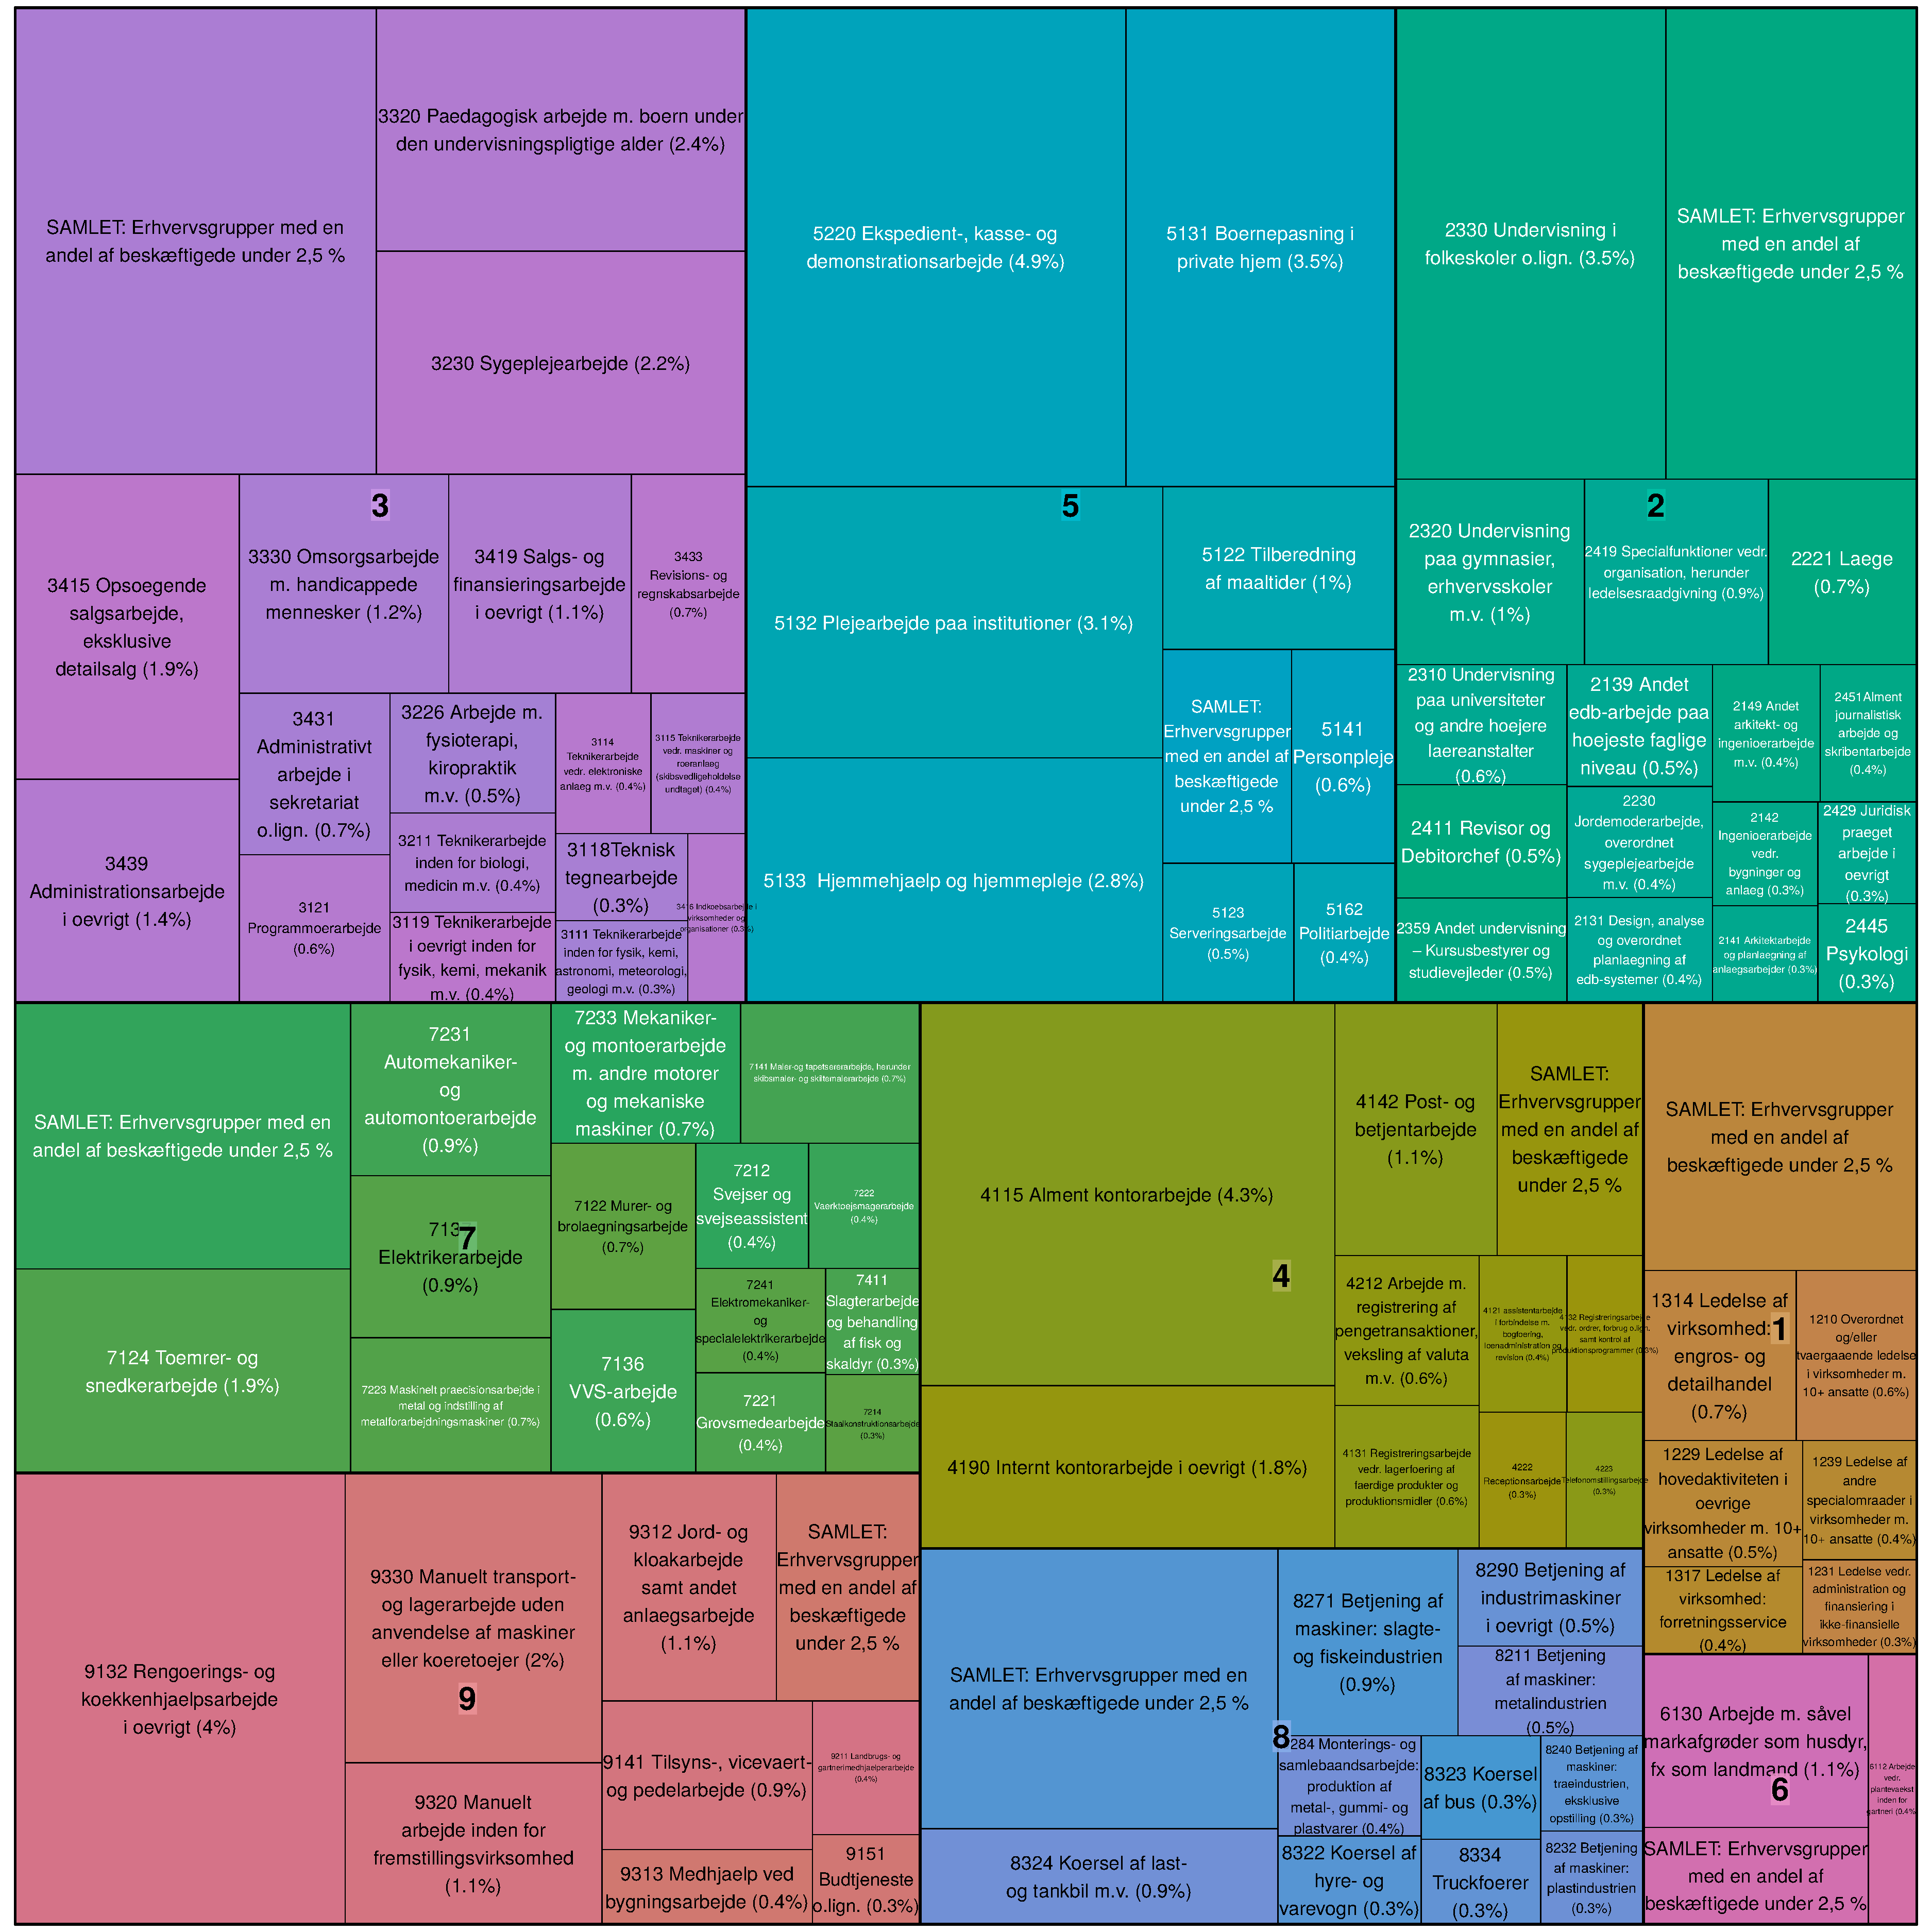
\includegraphics[width=1.0\textwidth]{fig/treemaps/DISCO_hovedgrp_beskaeft.pdf}
\end{center}
\end{figure}
\restoregeometry
%

Figuren skal forstås sådan, at den største DISCO-hovedgruppe befinder sig i øverste venstre hjørne, mens den mindste befinder sig i nederste højre hjørne. Vi ser, at hovedgruppe 3 indeholder den største andel af beskæftigede. Trækkortet viser os også, at erhvervsgrupperne i hovedgruppe 3 er meget diffentierede, lige fra \emak{d3230} til \emak{d3415}. 

Hvad trækortet også fortæller os, er at nogle erhvervsgrupper indeholder store dele af arbejdsmarkedet. \emak{d4115} indeholder f.eks. 4,3 \% af de beskæftigede, hvilket er næsten lige så meget som hele ledelshovedgruppe 1, og dobbelt så meget som hele landbrugshovedgruppe 6. 

indsæt evt boxplot med fordeling af discokoder her \#todo

%
\subsubsection{Bortfald og sager}
%

I en række tilfælde hvert år, er der personer, hvor ikke oplysninger på et 4-cifret DISCO-niveau. Disse findes i stedet på et 3-cifret eller 2-cifret niveau. Altså et mere overordnet, mindre detaljeret niveau. Disse er derfor at betragte som bortfald, da de ikke kan placeres i en 4-cifret kategori. 

Det gælder også de 4-cifrede kategorier, hvori antallet af observationer var for lavt til at retfærdiggøre deres egen erhvervsgruppe, og som ikke kunne slås sammen med andre kategorier. Jeg valgte at sætte grænsen til < 500 observationer%
%
    \footnote{ Det fjerner 72 kategorier, der indeholder 17.169 beskæftigede, svarende til 0,7 \% af populationen. Jeg vil mene det er et rimeligt tradeoff for en væsentlig reduktion i kompleksitet. Der er intet mønster i hvilke hovedgrupper disse 72 kategorier fjernes \emph{fra}. Dvs. det er ikke en bestemt \emph{type} arbejde, der derved udelades fra analysen.}%
%

Variablen \texttt{ANSXTILB} benyttes til at observere, om der er sket et skift i ansættelsesforholdene for den enkelte person siden sidste år \parencite{DST-ANSXTILB}. Det er centralt, da mange må formodes at opnå ansættelse indenfor samme beskæftigelse, og jeg derfor ikke kan benytte oplysninger fra \texttt{DISCO} alene: Det ville gøre det umuligt at vurdere, om der var tale om \emph{samme} ansættelse, eller en ny ansættelse indenfor samme job. Dette er endnu en kilde til bortfald: Det er ikke alle i populationen, der har udfald fra ANSXTILB i et eller flere år. Og det er ikke altid, at disse beskæftigelsesoplysninger stemmer overens med \texttt{DISCO}-koderne.    

Af de 313.073, der skifter jobs per år, er der et frafald på gennemsnitligt 33.653 observationer, hvor jeg kan se, at vedkommende \emph{har} skiftet job - men grundet ovennævnte årsager, er det ikke muligt at observere det som “et komplet jobskifte”, hvor ANSXFREM og DISCO-koderne hænger sammen på troværdig vis. Frafaldet blandt jobskiftere svarer til gennemsnitligt 10 \% pr år, hvilket jeg vurderer som ualarmenerende. 


Selvom bortfaldet i sig selv er beroligende lavt, så er det afgørende naturligvis, om der er systematik i hvem der bortfalder. En detaljeret bortfaldsanalyse, der ser på timelønninger helt ned på det 4-cifrede DISCO-niveau, findes i bilag \ref{app_loen}. Her konkluderer jeg, at lønniveauet i mit analyseudvalg ligger overordentligt tilfredsstillende tæt på lønniveauet i populationen, og at bortfaldet derfor ikke kræver særlige forbehold overfor de konklutioner, jeg fremlægger.  

% #todo du blir nok nødt til også at inkludere køn og alder i bortfaldsanalysen, hvis den sidste sætning der skal stå helt trovædigt.

% I figur \ref{figur metode disco frafald_beskaeft} ses det, at antallet af jobskiftere ligger ganske stabilt

% \begin{wrapfigure}{r}{8cm}
%   \vspace{-20pt}
%   \begin{center}
% \caption{Beskæftigelse, jobskifte og frafald i perioden 1996}
%    \label{figur metode disco frafald_beskaeft}
%     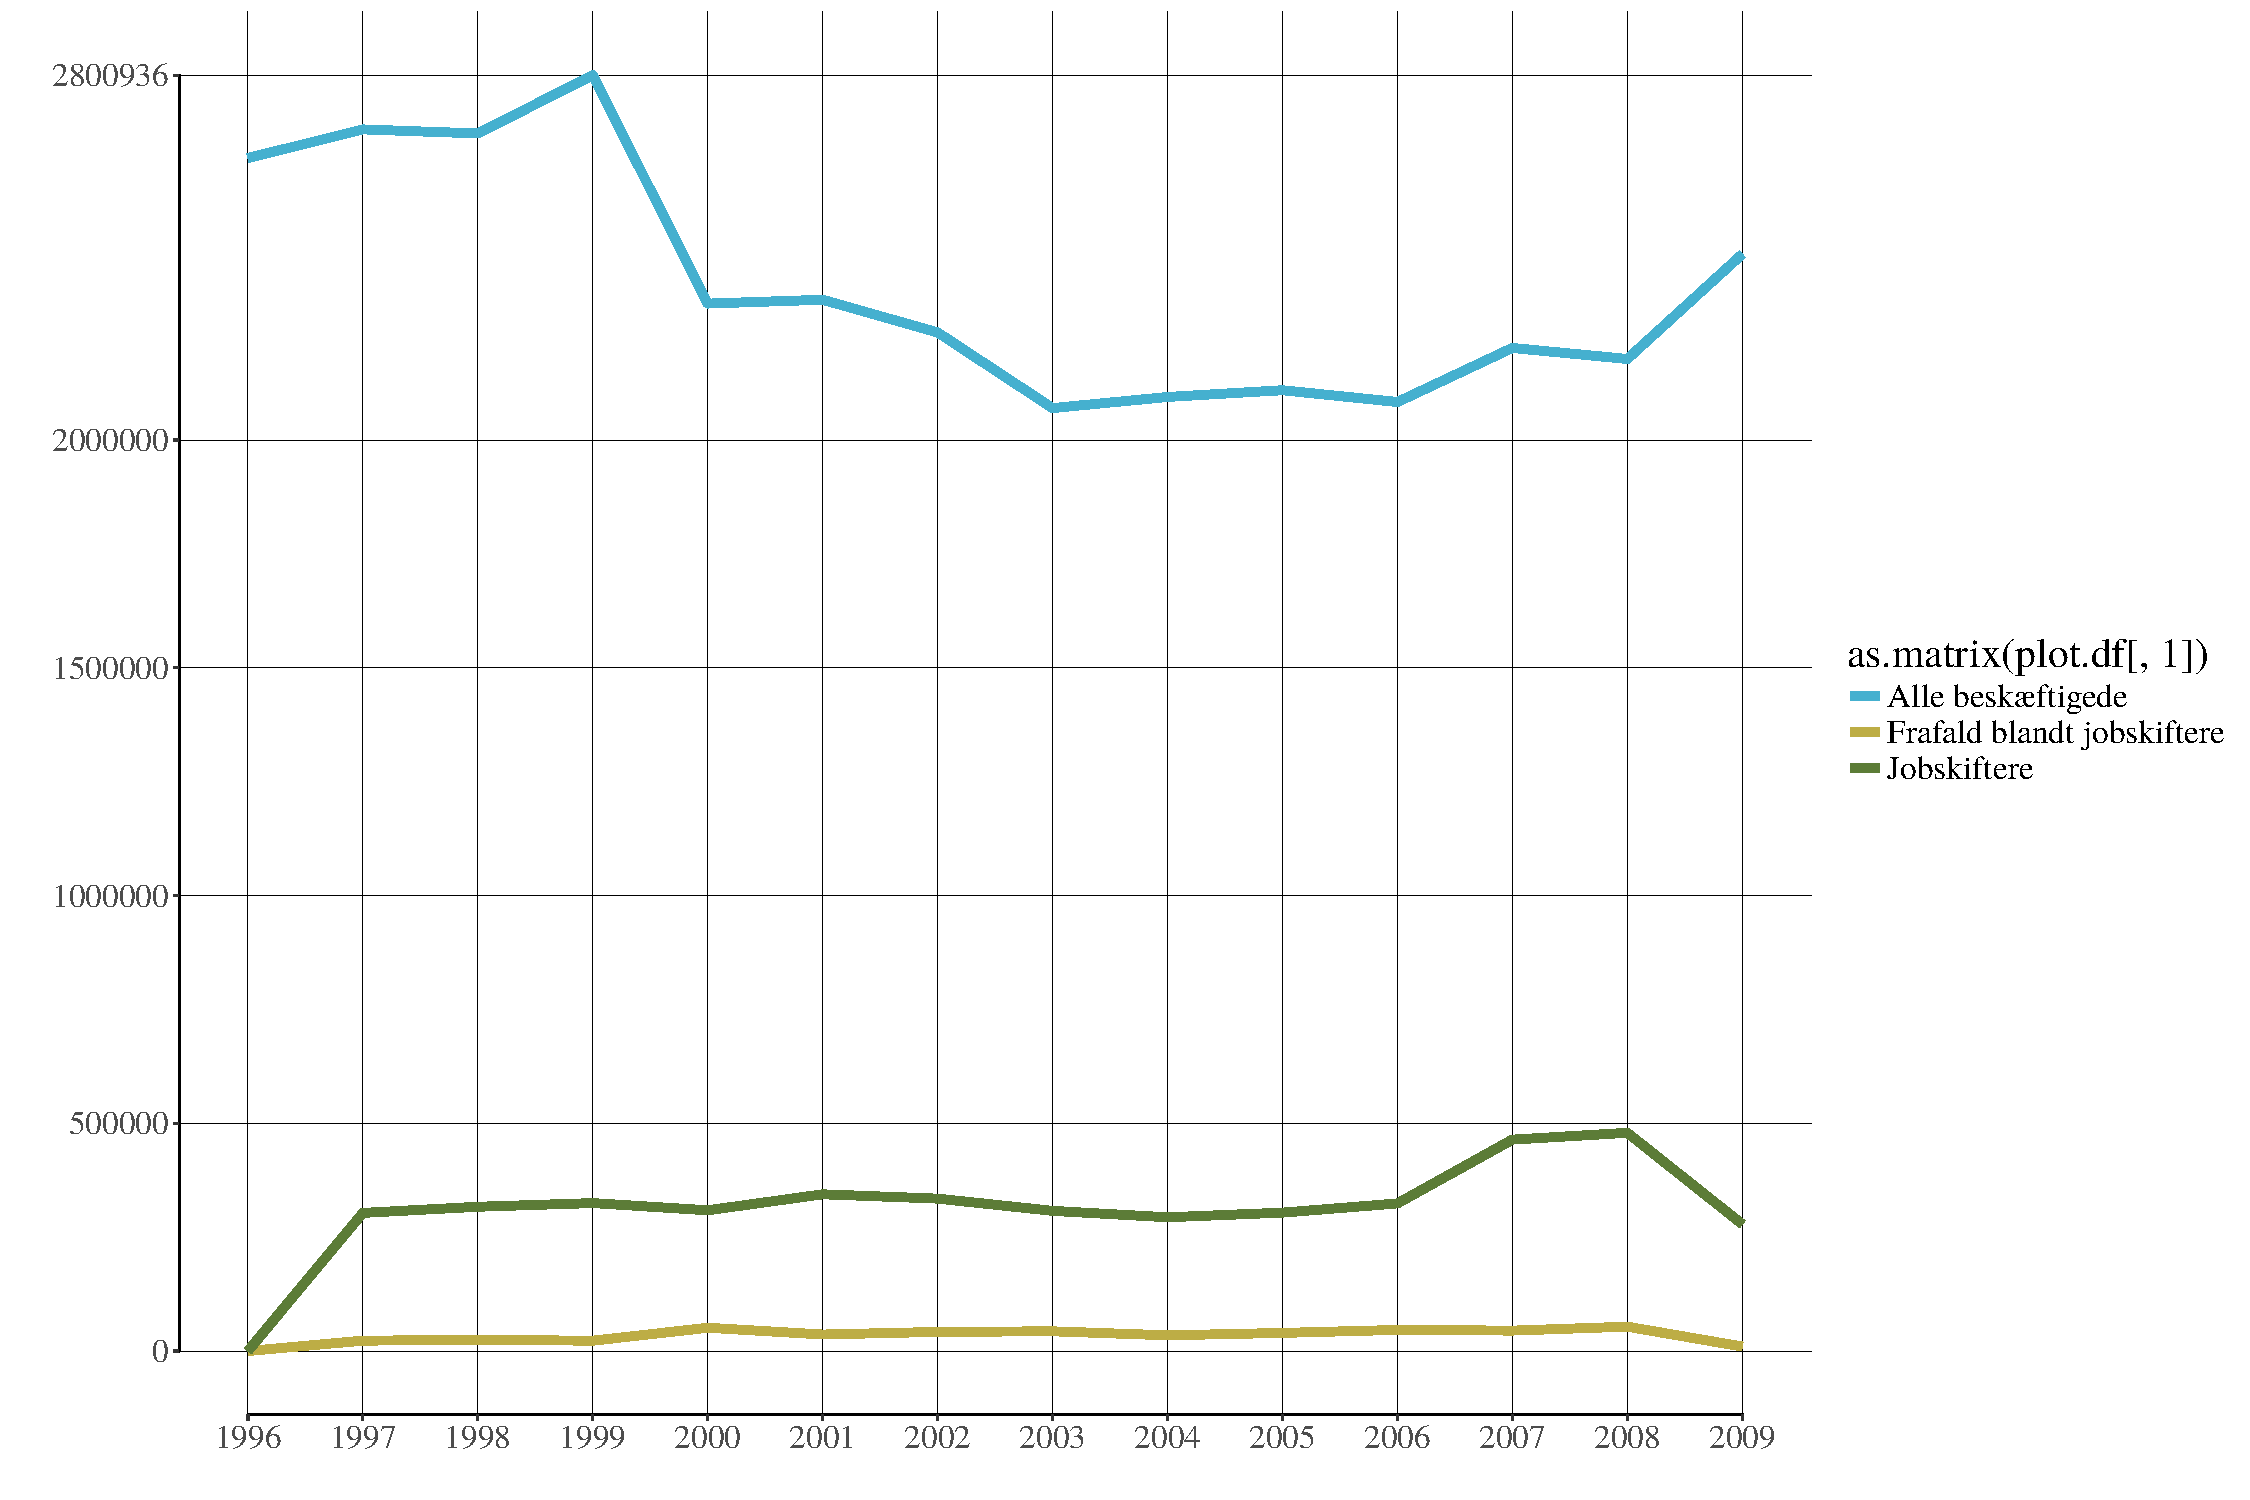
\includegraphics[width=8cm]{fig/tidsserier/frafald_beskaeft.pdf}
%     \label{fig_delanalyse1_kort_seg_proces2}
%   \end{center}
%   \vspace{-20pt}
% \end{wrapfigure}

% →  Det her hører til i bortfaldsanalysen, og ikke her. \#todo




%
\subsubsection{afrunding af DISCO}
%

For at lave segmenter a posteriori, foreslår MONECA-algoritmen grupperinger/klyngedannelser af \texttt{DISCO}-erhvervsgrupperne ud fra de reelle mobilitetsmønstre mellem jobs på arbejdsmarkedet. Dette kan i nogen grad sammenlignes med DISCOs 2- eller 3-cifrede niveau, bortset fra at det er ikke er baseret på en teoretisk klassificering af arbejdsfunktioner, men den reelle sociale logik, vi ser udspille sig i ansættelsesmønstre på arbejdsmarkedet.

Dette betyder for eksempel, at sundhedsvidenskabelige akademikere som farmaceuter, dyrlærer, læger og tandlæger ikke er et segment, fordi der ikke er nogen sammenhæng mellem bevægelserne mellem disse arbejdsstillinger, selvom de ifølge feltlogikken hos Danmarks Statistik har en høj grad af enshed i arbejdsfunktion samt færdighedsniveau. 


Det er det denne relle sociale logik, som den kommer udtryk gennem mobilitetsmønstre, næste afsnit vil omhandle. Først skal timelønninger dog berøreres, da det spiller så central en rolle i samfundet. q

%Den første hovedgruppe består af ledelse og fordeling af andres arbejde. Den anden hovedgruppe består  primært af akademisk arbejde, der typisk kræver en lang videregående uddannelse. Denn tredje hovedruppe består primært af personer med korte og mellemlange videregående uddannelser indenfor en lang række erhverv.  De fire hovedgrupper næste består af personer med færdigheder, der, \emph{rent formelt} i uddannelsessystemet, kræver grundskoleuddannelse,  grundskolen, erhvervsskole og gymnasieskolerne og den sidste består af arbejdsstillinger som ikke k


%%%%%%%%%%%%%%%%%%%%%%%%%%%%%%%%%%%%%%%%%%%%%%%%%%%%%%%%%%%
\section{Timeløn}
%%%%%%%%%%%%%%%%%%%%%%%%%%%%%%%%%%%%%%%%%%%%%%%%%%%%%%%%%%%

Jeg benytter indkomstvariablen timeløn. I bilag \ref{app_loen} beskriver jeg variablen samt den datarensning jeg foretager, samt sammenligner den med de andre mulige indkomstvariable og DSTs egne mål for indkomst for forskellige erhvervsgrupper. De væsentlige pointer fra bilaget er:
%
 \begin{itemize}
  \itemsep -0.5em
  	\item Timelønsvariablen er det bedste skøn på indkomst, og er ganske nøjagtigt selv på mit detaljerede \texttt{DISCO}-niveau.
  	\item Medmindre andet siges, er timelønninger \emph{et gennemsnit} af lønningerne i hele perioden 1996-2009. I beregningen af dette gennemsnit er perioden 1996-2008 inflationskorrigeret til 2009 priser.
  	\item Månedslønninger beregnes ved at gange timelønnen med 160,33. Det er DSTs metode \parencite[32]{DST2009}.
 \end{itemize}
%
Når man undersøger sit eget forslag til arbejdsmarkedsstruktur skal man være opmærksom på, at det ikke kan valideres med ved hvad Boje kalder “outcomes af sociale processer,” såsom arbejdsløshed, hyppighed i jobskift og, ikke mindst: lønforskelle \parencite[28]{Boje1985}. Det er indkomst og indkomstforskelle mellem delmarkederne, jeg vil gennemgå nu. 

I netværksmetodologiske termer er Laumann, Marsden \& Prensky inde på det samme, når de advarer imod at validere et socialt netværk baseret på de selvsamme attributter, der er brugt til at konstruere det \parencite[29]{Laumann1983}. Løn er ikke brugt til at konstruere mit netværk, men må siges at være så tæt et outcome af beskæftigelse, at det ikke fremstår eksternt i Lauman et als (skriver man det sådan? \#todo) forstand. Lønniveauerne på de af Moneca skabte \emph{delmarkeder} er derimod interessante for validiteten, hvis vi accepterer det som et \emph{kriterie-relateret validitetsmål}, der gør det muligt at validere den interne struktur og konsistens i et klasseskema \parencite[94]{Oesch2006a}%
%
\footnote{ Jeg laver ikke et klasseskema, men er tæt nok på til jeg synes det giver mening at benytte Oeschs validitetskriterie.}%
%
. Udover denne mere metodologisk nødvendige validering af mit bud på en segmenteringsstrukur, er lønninger \emph{i sig selv} interessante, da det er direkte relaterbart til arbejdsmarkedets struktur, og utvivlsomt er den mest benyttede indikator for social status og magtposition i den sociale struktur Oesch \parencite[95]{Oesch2006a}. %s. 95, (Weber, Andrade, Boje, Marx, Wright, Goldthorpe, Harrits, Scott - find dem og skriv dem ind, fx \#todo.) 





%%%%%%%%%%%%%%%%%%%%%%%%%%%%%%%%%%%%%%%%%%%%%%%%%%%%%%%%%%%
\section{Køn}
%%%%%%%%%%%%%%%%%%%%%%%%%%%%%%%%%%%%%%%%%%%%%%%%%%%%%%%%%%%


%%%%%%%%%%%%%%%%%%%%%%%%%%%%%%%%%%%%%%%%%%%%%%%%%%%%%%%%%%%
\section{Ledighed}
%%%%%%%%%%%%%%%%%%%%%%%%%%%%%%%%%%%%%%%%%%%%%%%%%%%%%%%%%%%


%%%%%%%%%%%%%%%%%%%%%%%%%%%%%%%%%%%%%%%%%%%%%%%%%%%%%%%%%%%
% \fi
%Local Variables: 
%mode: latex
%TeX-master: "report"
%End: